\documentclass{beamer}
\usetheme{CambridgeUS}
\usecolortheme{rose}
\usepackage{amsmath,amsthm,amssymb,amsfonts,latexsym}
\usepackage[notocbib]{apacite}
\usepackage[english]{babel}
\usepackage[applemac]{inputenc}
\usepackage{caption}
\usepackage{graphicx}
\usepackage{enumerate}
\usepackage{array}
\usepackage{color}
\usepackage{caption}
\usepackage{pdflscape}
\usepackage{hyperref}
\captionsetup{labelformat=simple}
\usepackage{arydshln}
\usepackage{booktabs}
\usepackage{comment}
\newtheorem{proposition}[theorem]{Proposition}
\newcolumntype{H}{>{\setbox0=\hbox\bgroup}c<{\egroup}@{}}
\newcommand{\tick}{\ding{52}}

\definecolor{darkgreen}{RGB}{6,101,0}
\definecolor{wine}{RGB}{135,0,0}
\definecolor{'darkgray'}{gray}{0.35}

\setbeamertemplate{blocks}[rounded][shadow=false]

\DeclareMathOperator{\Var}{Var}
\DeclareMathOperator{\E}{E}

\title[Reelection Backfire]{Reelection Backfire: \\ Political Accountability and Security Under-provision in Mexico}

\author[rafael.ch@nyu.edu]{ $\underset{\text{\it NYU}}{\text{Rafael Ch}}$} 

\date[]{}
\institute[]{}

\begin{document}

\frame{\titlepage}
%Frame_____________________________________________________________________

\begin{frame}[label=introduction]{Introduction}

\begin{itemize}  
	 		  \setlength\itemsep{0.4em} 
\item Reelection: \textcolor{blue}{Mayhew's (1974)} ``electoral connection" - incumbent's behavior constrained by reelection desire
	\begin{itemize}
	\item  widespread among democratic representative systems 
	\item 80s, 90s: go-to policy recommendation to foster political accountability
	
	\end{itemize}
\item \alert{However,} conflicted evidence on the effect of term limit removal
\item Positive side:
	\begin{itemize}
	\item $\uparrow$ competence of elected politicians (\textcolor{blue}{Dalbo et. al 2017})
	\item $\downarrow$ corruption (\textcolor{blue}{Ferraz \& Finan 2008, 2011})
	\item $\uparrow$ legislators productivity (\textcolor{blue}{Hall et. al 2018})
	\item $\uparrow$ welfare (\textcolor{blue}{Alt et. al 2011})
	\end{itemize} 
\item Negative side:
	\begin{itemize}
	\item $\uparrow$ particularistic legislation (\textcolor{blue}{Motolinia 2020})
	\item $\uparrow$ corruption (\textcolor{blue}{Coviello et. al 2017}) %due to longer tenuer  
	\end{itemize} 
\item At face value: reelection does not always lead to \underline{political} \underline{accountability} for the median voter 
\end{itemize}


\end{frame}
%_____________________________________________________________________
\begin{frame}[label=question] 
\begin{itemize}
	\item What features limit the political accountability of reelection?
	 \\[5pt]
\textit{\textcolor{blue}{Such as parties' electoral incentives}}
	\bigskip
\item
\alert{This is the focus of this paper.}
\end{itemize}
	
\end{frame}
%_____________________________________________________________________
\begin{frame}[label=this_paper]{This paper}
 
Studies:
\begin{itemize}	
 		  \setlength\itemsep{1em} 
	
	\item Effect of term limit removal on violence (proxy  welfare distortion) and public security provision (incumbents' effort) \hyperlink{why_security}{\beamerbutton{Why public security?}}

	\item Leverage staggered implementation of 2014 Term Limit Reform in Mexico  \hyperlink{why_mexico}{\beamerbutton{Why Mexico?}} 

		\begin{itemize}
		\item Reelection for 2 consecutive periods for local executives
		\item Staggered implementation at state-level from 2015 to 2022
		\end{itemize}
		
	\item Effect of reelection on incumbent party electoral incentives

	    \begin{itemize}
		\item \textcolor{blue}{Samuels \& Shurgart (2010)}: mayors as agents to parties and voters, accountability and delegation tension
		\item \textcolor{blue}{Berman \& Lake (2019)}:``Why principals deviate from optimal control of agents [in charge of deterring non-state challengers]?"
		\end{itemize}

\end{itemize}

	 
\end{frame}

%_____________________________________________________________________
\begin{frame}[label=preview]{Preview of main results}

\begin{itemize}
 		  \setlength\itemsep{1em} 

	\item Event-study design shows term limit removal led under-provision of public security by military and local police forces
	% \item Stronger effect in the presence of security cooperation agreements among different levels of gov.
		\begin{itemize}
			\item \alert{Result: increase violence treated municipalities}
		\end{itemize}

	\item Not explained by: (1) adverse candidate selection, (2) citizens security preferences, (3) capture by DTOs
	\item Robust to:
		\begin{itemize}
		\item Multiple homicide databases
		\item Sensitivity analysis pretrend violation
		\item Falsification of treatment
		\end{itemize}
\end{itemize}
	
\end{frame} 
%_____________________________________________________________________
\begin{frame}[label=preview_mechanisms]{Preview of mechanism}

RDD \& Event-in-discontinuity of close elections designs: 
\begin{itemize}
	\item Reform generated an incumbency avantage
	\item Increase prob. of survival reduced party monitoring of local agents that tackle crime (military \& police forces)
\end{itemize}
\bigskip
Strategic behavior:
\begin{itemize}
	\item PRI followed a ``not in my backyard strategy"
	\item Targeted security efforts in opposition municipalities making them bare the externalities of the War on Drugs
	\item Violence increased in opposition municipalities relative to PRI ones
\end{itemize}
\bigskip
 
%But what about voter accountability then? Yields public security \& violence reduction only if
%	\begin{itemize}
%	\item electoral competition is substantially high 
%	\item mayor is fully in control of public security provision
%	\end{itemize}
\end{frame} 



%_____________________________________________________________________
\begin{comment}
	
\begin{frame}[label=war_drugs]{From here on...}

\begin{enumerate}
 
	\item Argument
	\item War on Drugs in Mexico
	\item 2014 Term Limit Reform 
	\item Research Design
	\item Main Results
	\item (rule out) Alternative explanations
	\item Mechanisms
	\item Policy recommendations
\end{enumerate}
 
	
\end{frame} 
\end{comment}

%_____________________________________________________________________

\begin{frame}[label=argument]{Argument}

\begin{itemize}
 		  \setlength\itemsep{1em}
	
	\item  Since \textcolor{blue}{Mayhew 1974}, large literature on political accountability effect of reelection
	\item But ``electoral connection" states that reelection is maximized by catering particularistic transfers. Salient when
		\begin{itemize}
		\item Parties suffer political misfortunes (\textcolor{blue}{Motolinia 2020})
		\item Clientelistic parties (\textcolor{blue}{Fergusson et. al 2018})
		\end{itemize} 
	\item Result: longer tenure associated with particularistic transfers and corruption (\textcolor{blue}{Coviello et. al 2017}) 
	\item Another limit to the political accountability of reelection:
	\begin{itemize}

	\item 
	\alert{Incumbent party political survival} %triggers weak oversight}
	\end{itemize} 

\end{itemize} 
	 
\end{frame} 
%_____________________________________________________________________
\begin{frame}[label=survival]{Political survival}

\begin{itemize}
 		  \setlength\itemsep{0.5em}
	
	\item Incumbents are accountable to voters and political parties: two principals-agent problem (\textcolor{blue}{Moreno et. al 2003, Samuels \& Shugart, 2010, Klasnja \& Titiunik, 2017})
	\item Top-down accountability=f(party strength, party electoral incentives)
	\begin{enumerate}
		\item Party strength: ability to monitor
		\item Electoral incentives: willingness to monitor
	\end{enumerate}
	\item Electoral incentives: party able but not willing to monitor
	\item Mexico: assume strong party strength
		\begin{itemize}
		\item \alert{Increase party political survival $\rightarrow$ weak oversight} 
		\end{itemize}

	\item E.g. incumbency advantage. \textcolor{blue}{Weaver 2020} appears when
		\begin{itemize}
		\item voters don't associate first term in office with experience on corruption
		\item believe strong horizontal or vertical accountability institutions to oversight incumbents
		\end{itemize}
	
\end{itemize} 
	
\end{frame} 
%_____________________________________________________________________
\begin{frame}[label=hypotheses]{Hypotheses}

\begin{itemize}
 		  \setlength\itemsep{1em}
 
	\item \textbf{H1:} $\uparrow$ political survival principal (inc. advantage) $\rightarrow$ $\downarrow$ oversight of agent
	
	\item \textbf{H2:} $\downarrow$ oversight $\rightarrow$ $\downarrow$  agent's effort (security provision)
	
	\item \textbf{H3:} $\downarrow$ effort (security provision) $\rightarrow$ $\uparrow$ welfare distortions (violence)
	
\bigskp

\item \textbf{Accountability paradox:} under strong parties, reelection leads voters to create an incumbency advantage, while the advantage decreases the willingness of parties to do so

\end{itemize} 
	
\end{frame} 

%_____________________________________________________________________

\begin{frame}[label=war_drugs]{Mexico's War on Drugs}
 
\begin{itemize} 
 		  \setlength\itemsep{0.5em}
  
	\item From 2006-2019: more than 300,000 deaths and more than 30,000 forced disappearances  
	\item Reasons:
		\begin{itemize}
		\item DTOs drug markets competition (\textcolor{blue}{Rios 2013})
		\item State effort to reduce DTOs operations (\textcolor{blue}{Rios 2013, Dell 2015})
		\item Cocaine supply shortages (\textcolor{blue}{Castillo et. al 2018})
		\end{itemize}
\item Multiple pacification strategies tested:
		\begin{itemize}
		\item beheading drug kingpins
		\item deployment of troops (45,000)
		\item increasing military \& police capacity (e.g. Plan Merida)
		\item corruption detection \& money laundering policies
		\item increase fiscal transfers for crime prevention
		\item security cooperation agreements (e.g. Mando \'Unico)
		\item financing self-defense groups (most effective but generate stateless)
		\item \alert{strengthening political accountability ???}
		\end{itemize}
\end{itemize} 
	
\end{frame} 

%_____________________________________________________________________
\begin{frame}[label=reform_content]{2014 Term Limit Reform: content}

 \hyperlink{reform_background}{\beamerbutton{Reform Background}} 
 
 Proposed three main changes:
\begin{enumerate}
	\item Creation of INE
	\item Term limit removal of mayors for 2 consecutive terms (also legislators for more terms)
	\item Party-lock: those running for reelection could not switch parties
\end{enumerate}
\bigskip
On staggered treatment timing: 
\begin{itemize}
	\item state legislatures (under governors control) granted discretion to define...
	\begin{enumerate}
	\item number of terms 
	\item implementation date (could not affect 2014 elections by law)
	\end{enumerate}  
\end{itemize}
 
\end{frame} 
%_____________________________________________________________________
\begin{frame}[label=reform] 
\begin{figure}[H]   
\centering 
\caption{Mexican States Electoral Reform Treatment Status}
\label{fig:treatment_status}
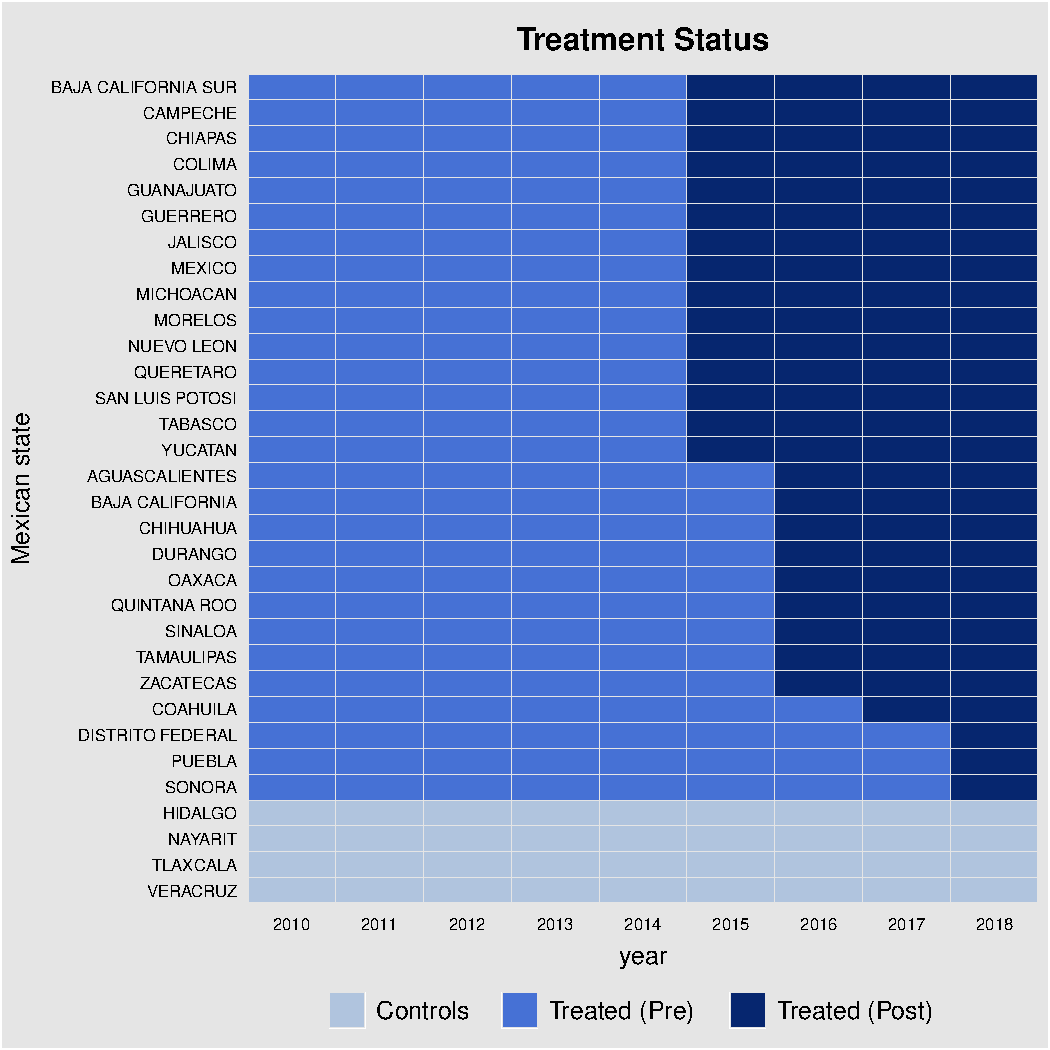
\includegraphics[width=0.6\textwidth]{Figures_pres/reform_treatmentstatus.pdf}     
\captionsetup{justification=centering} 
\end{figure}      

\end{frame} 
%_____________________________________________________________________
\begin{frame}[label=data]{Data}
 
 \begin{itemize}
 		  \setlength\itemsep{1em}
	
 	\item  Database on violence and effort by military and local police forces
 	\item Unit: municipalities from 2010 to 2018
 	\item Main outcome: Homicides to proxy for violence
 		\begin{itemize} 
 		\item INEGI's homicide related deaths
 		\item SNSP's homicides (counts cases; for robustness)
 		\item Population: INEGI and CONAPO projections
 		\item logged and inverse hyperbolic sine (IHS) transformation %(\textcolor{blue}{Mackinnon \& Maggie, 1990})
 		\end{itemize}
 		
 	\item Mechanisms: 
 		\begin{itemize} 
 		\item Military's effort: narcotics, arms and laboratories erradicated 2010-2018 (INFOMEX)
 		\item Police's effort: criminal detentions 2010-2018 (INFOMEX)
 		\item Incumbency advantage: 
 			\begin{itemize} 
 			\item Incumbent $t-1$, barely winning (loosing) at $t$, on election outcome at $t+1$ (\textcolor{blue}{Klasnja \& Titiunik, 2017})
 			\item State \& municipal winning margin (\textcolor{blue}{Magar, 2012, 2017})

 		 	\end{itemize}

 		\end{itemize}
 \end{itemize}


\end{frame} 
%_____________________________________________________________________
\begin{frame}[label=design]{Research Design}
\begin{itemize}
	\item Cohort weighted event-study design (\textcolor{blue}{Abraham \& Sun, 2020}):
	%\item Exploit staggered implementation of reform

 \begin{equation}
 \label{eq:abraham} 
\begin{split}
$y_{mt}=\mu_m + \mu_t + \sum^{5}_{e=1} \sum^3_{k=-7, \neq {-8,-1}} \gamma_{e,k}(1\{E_i=e\} \cdot R^k_{m,t})$ \\
 $+ \sum^{5}_{e=1} \sum^3_{k=-7, \neq {-8,-1}}  \Theta'X_{s(m)t} (1\{E_i=e\} \cdot R^k_{m,t}) + \epsilon_{mt}$ 
\end{split}   
\end{equation} 

%where
\begin{itemize}
 		  \setlength\itemsep{0.3em} 
  
	\item $y_{mt}$: log/ihs(homicides per capita), log(anti-narcotic operations) 
	\item exclude  $\gamma_{-8,-1}$ to avoid collinearity
	\item $\mu_m$ \& $\mu_t$: municipality and year FEs
	\item $E_i$: cohort-specific indicators
	\item $R^k_{m,t}$: Term Limit Reform indicator
	\item $X_{s(m)t}$: state $s$ (municipal $m$) level covariates
	\item $\gamma_{e,k}$: DiD estimators or Cohort Average Treatment Effects (CATTs).
	\item SEs clustered state-level (Reform treatment level)
	
\end{itemize} 
\end{itemize}

\end{frame}

%_____________________________________________________________________
\begin{frame}[label=iw_estimators]{Main estimators}
\begin{itemize}
 		  \setlength\itemsep{0.5em}   

	%\item Take linear combination of the CATTs for each relative time period $k$
	%\item Weight each cohort by relative share of the sample
	\item Construct interaction weighted (IW) estimators (\textcolor{blue}{Abraham \& Sun, 2020})
	%\item Exploit staggered implementation of reform

 \begin{equation}
\hat{\nu}_g=\frac{1}{|g|}\sum_{k \in g}\sum_e \hat{\gamma_{e,k}} \hat{Pr}\{E_i=e | E_i \in [-k, T-k]\}	 
\end{equation} 
 
\begin{itemize}
\item $\hat{\gamma_{e,k}}$: CATTs returned from equation (\textcolor{blue}{\ref{eq:abraham}})  %(\textcolor{blue}{1})      
\item $\hat{Pr}\{E_i=e | E_i \in [-k, T-k]\}$: estimated cohort weights
\item estimator normalized by the size of  $g$
\item $\hat{\nu}_g$: weighted linear combination of the CATTs
\end{itemize}

\end{itemize}

\end{frame}
%_____________________________________________________________________
\begin{frame}[label=main_results]{Main results}
\begin{figure}[h] 
\centering
\caption{Effect of Term Limit Reform of 2014 on Violence, IW estimators with 95\% confidence intervals}
\label{fig:event_study_log}
 
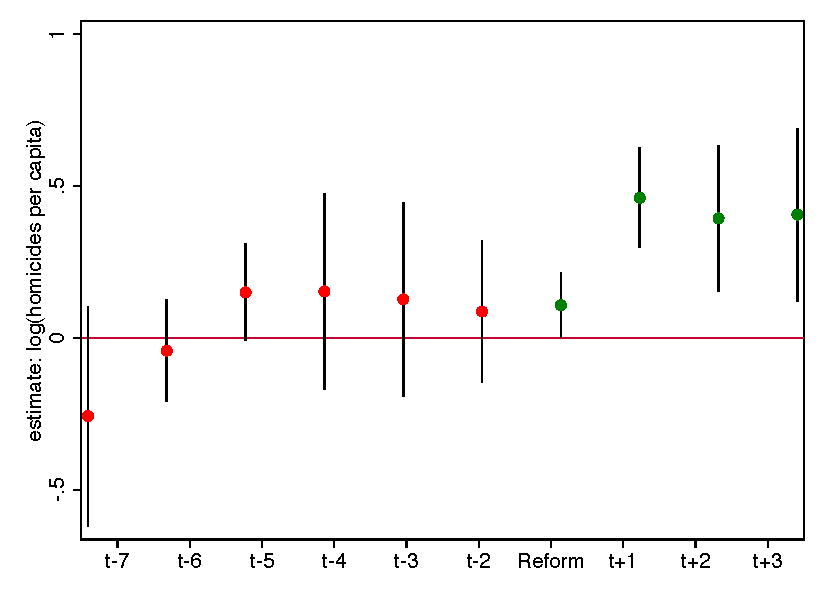
\includegraphics[width=0.65\textwidth]{Figures_pres/event_study_log.pdf}
       \captionsetup{justification=centering}

 %{\footnotesize Note: IW estimators for each lead and lag relative to the first year of treatment.} 
 \hyperlink{ihs_results}{\beamerbutton{IHS transformation}} 

\end{figure}   

\end{frame}
%_____________________________________________________________________
\begin{comment}
	
\begin{frame}[label=identification]{Identification}
Four identifying assumptions: 
\begin{enumerate}
 		  \setlength\itemsep{1em}   
	\item Pretrends, and given CATTs no bias from other relative timer periods
	\item {\it As-if} random assignment of treatment
	\begin{itemize}
		\item Strong assumption given governors potential selection bias
		\item Include governors' strength covariates: winning margin and partisan alignment with central government
		\item ID assumption now: conditional on covariates and FEs, unobserved factors are not correlated with Reform treatment assignment
	\end{itemize}
	\item No anticipatory behavior of agents
		\begin{enumerate}
		\item Assume it can only occur in fixed window prior to Reform; but late adopters could anticipate
		\item No difference between late and early adopters \hyperlink{event_by_event}{\beamerbutton{Event-by-event analysis}} 
	\end{enumerate}
  
 %\item \textcolor{white}{No treatment effect heterogeneity accounted by cohort weighted event-study design}

\end{enumerate}

\end{frame}
\end{comment}


%_____________________________________________________________________
\begin{frame}[label=identification2]{Identification}
Four identifying assumptions: 
\begin{enumerate}
 		  \setlength\itemsep{0.5em}   
	\item Pretrends, and given CATTs no bias from other relative timer periods
	\item {\it As-if} random assignment of treatment
	\begin{itemize}
		\item Strong assumption given governors potential selection bias
		\item Include governors' strength covariates: winning margin and partisan alignment with central government
		\item ID assumption now: conditional on covariates and FEs, unobserved factors are not correlated with Reform treatment assignment
	\end{itemize}
	\item No anticipatory behavior of agents
		\begin{enumerate}
		\item Assume it can only occur in fixed window prior to Reform; but late adopters could anticipate
		\item No difference between late and early adopters \hyperlink{event_by_event}{\beamerbutton{Event-by-event analysis}} 
		\end{enumerate}
 
 \item No treatment effect heterogeneity accounted by cohort weighted event-study design (\textcolor{blue}{Abraham \& Sun, 2020}): 
 		\begin{itemize}
		\item \alert{Saturated FEs structure: treatment units do not enter test window as control units} 
		\end{itemize}
\end{enumerate}
\bigskip 
%\centering 
%\alert{Unbiased positive causal effect of reelection on violence}
\end{frame}
%_____________________________________________________________________
\begin{frame}[label=robustness]{Robustness tests}
\begin{enumerate}
 		  \setlength\itemsep{1em}   
	\item Test different homicide databases  \hyperlink{diff_datasets}{\beamerbutton{Different datasets}} %pretrends and positive effects found    
	\item Sensitivity analysis on potential violations of parallel trends (\textcolor{blue}{Rambachan \& Roth, 2019)}   \hyperlink{sensitivity_analysis}{\beamerbutton{Sensitivity analysis}} 
			%\begin{itemize}
			%\item Sensitivity analysis on parallel trend violation incorporating context specific knowledge   \hyperlink{sensitivity_negative}{\beamerbutton{Decreasing violation}}  \hyperlink{sensitivity_positive}{\beamerbutton{Increasing violation}}
			%\end{itemize}
	\item Falsification test: randomly assign Mexican states to treatment, keeping observed proportion of treated units per year  \hyperlink{falsification}{\beamerbutton{Falsification}}   
	\item Asymmetric effects when accounting for security cooperation agreements \hyperlink{mando_unico}{\beamerbutton{Coop. Agreements}} 
		\begin{itemize}
		\item Effect persist after controlling for coop. agreements \hyperlink{mando_unico_control}{\beamerbutton{Coop. Agreements control}} 
		\end{itemize}
\end{enumerate}   

\end{frame}
%_____________________________________________________________________
\begin{frame}[label=mechanism_design]{Inc. Advantage: Event study-in-discontinuity of close elections design}
\begin{itemize}
	\item Local linear regression for municipalities in an \textcolor{blue}{Imbens-Kalyanaraman} optimal bandwidth: 
 \begin{equation}
\begin{split} 
$y_{mt}=\mu_m + \mu_t + \sum^5_{e=1} \sum^0_{k=-5, \neq {-6,-1}} \gamma_{e,k}(1\{E_i=e\} \cdot R^k_{m,t})$ \\ 
$+ \sum^5_{e=1} \sum^0_{k=-7, \neq {-5,-1}}  \Theta'X_{it} (\mathbbm{1}(E_i=e)\cdot R^k_{m,t}) + f_{(.)}(margin)_{mt}$ \\
 $+ \sum^5_{e=1} \sum^0_{k=-5, \neq {-6,-1}} \nu_{e,k}(1\{E_i=e\} \cdot R^k_{m,t} \cdot  f_{(.)}(margin)_{mt} )+ \epsilon_{mt}$  
\end{split}   
\end{equation}  
%where
	\begin{itemize} 
 		  \setlength\itemsep{0.1em} 
	\item $f_{(.)}(margin)_{mt}$: RD polynomial on winning margin
	\item $k$ relative time periods run from  $k \in\{-6,-5,...,0\}$
	\item exclude  $\gamma_{-6,-1}$ to avoid collinearity; $\gamma_{-2}$ non-existent 
	\item $\gamma_{e,k}$: CATTs
	\item SEs clustered state-level (treatment level)
	\end{itemize} 

\end{itemize}
 
\end{frame}   

%_____________________________________________________________________
\begin{frame}[label=incumbency_advantage]{Incumbency Advantage}
\begin{figure}[h] 
\centering
\caption{Effect of Term Limit Reform of 2014 on Incumbency Advantage, IW estimators with 95\% confidence intervals}
\label{fig:incumbency_adv_1234}
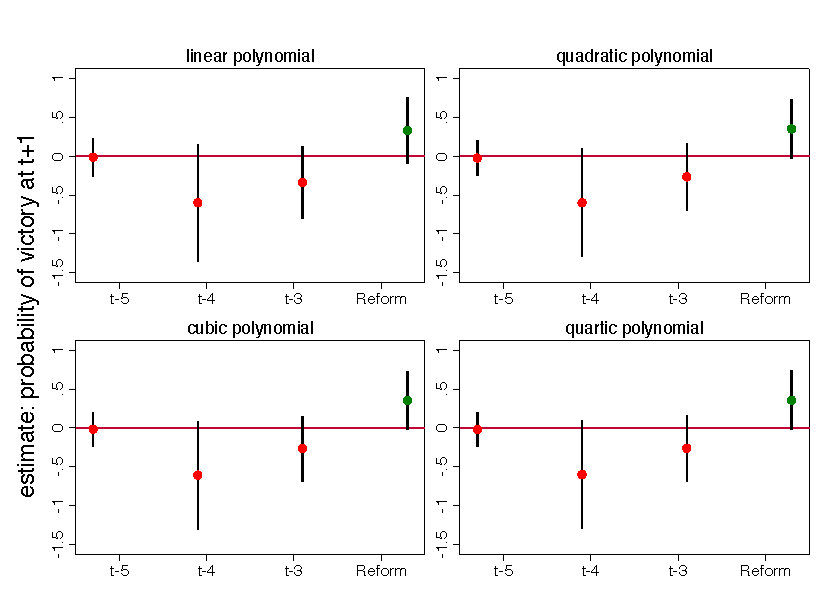
\includegraphics[width=0.73\textwidth]{Figures_pres/incumbency_advantage_234.pdf}
       \captionsetup{justification=centering}

 %{\footnotesize Note: IW estimators for each lead and lag relative to the first year of treatment.} 
 %\hyperlink{ihs_results}{\beamerbutton{IHS transformation}} 

\end{figure} 
\end{frame}
%_____________________________________________________________________
\begin{frame}[label=mechanism_identification]{Inc. Advantage: Identification}
\begin{itemize}
	\item Close elections where party barely won to those where it barely lost: isolate from current and future electoral success
	\item DiD setup: tease time-variant and time-invariant confounding variation
	\item Identification assumptions: 
	\begin{enumerate}
		\item pretrends (found)
		\item as-if random treatment assignment (conditional on covariates)
		\item no anticipatory behavior  \hyperlink{event_by_event_figure2}{\beamerbutton{Event-by-event analysis}}
		\item treatment effect homogeneity (CATTs)
		\item selection into treatment
		\begin{itemize}
		\item no covariate jump at discontinuity \hyperlink{population}{\beamerbutton{Population}} 
		\item density test \hyperlink{mccrary_test}{\beamerbutton{Mccrary Test}} 
		\end{itemize} 
	\end{enumerate} 
\item Similar results using RDD design \hyperlink{rdd_figure}{\beamerbutton{RDD figure}} \hyperlink{rdd_table}{\beamerbutton{RDD table}} 
 

\end{itemize}
 
\end{frame} 

%_____________________________________________________________________
\begin{frame}[label=effort_security]{Effort placed by Security Forces}

\begin{figure}[h] 
\centering 
\caption{Effect of Term Limit Reform of 2014 on Security Forces Effort, IW estimators with 95\% confidence intervals}
\label{fig:effort_security}
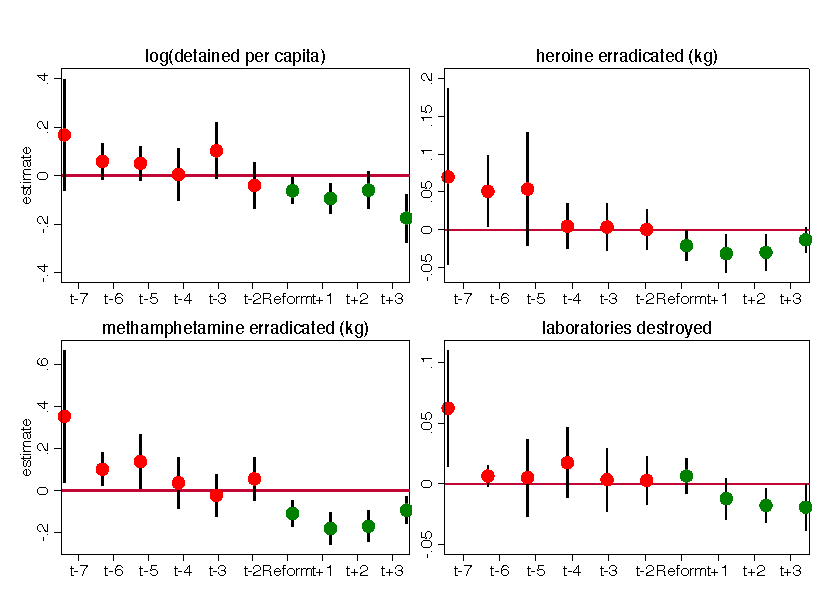
\includegraphics[width=0.73\textwidth]{Figures_pres/effort_security.pdf}
       \captionsetup{justification=centering}

 %{\footnotesize Note: IW estimators for each lead and lag relative to the first year of treatment.} 
 %\hyperlink{ihs_results}{\beamerbutton{IHS transformation}} 
 
\end{figure}  

\end{frame}
%_____________________________________________________________________
\begin{frame}[label=effort]{Strategic placement of effort by security forces}

\begin{itemize}
 		  \setlength\itemsep{1em}   
	
	\item Concern that rampant crime hides a non-strategical choice by security forces
	\item Heterogeneous treatment effects show this is not the case:
	\begin{enumerate}
	 		  \setlength\itemsep{0.5em}   
		\item \hyperlink{strategic1}{\beamerbutton{Party Alignment:}} aligned municipalities with PRI central government show a decrease in violence  
		\item \hyperlink{strategic2}{\beamerbutton{``Not in my backyard" strategy}}: low security provision in PRI municipalities, and high in opposition ones (PAN and MORENA)  
		\item \hyperlink{strategic3}{\beamerbutton{``Let others burn" strategy}}: increase of violence in opposition municipalities 
		\begin{itemize}
		\item Importance negative externalities of War on Drugs
		\end{itemize}
	\end{enumerate} 
\end{itemize}
	
\end{frame}

%_____________________________________________________________________
\begin{frame}[label=alternative_explanations]{(ruling out) Alternative Explanations}

\begin{enumerate}
 		  \setlength\itemsep{1em}   

	\item Adverse politician selection: positive and non-significant effect of Reform on incumbent's quality \hyperlink{quality}{\beamerbutton{Incumbents quality}} 
	\begin{itemize}
		\item quality: web-scrape mayors' professional titles from 2010-2019 from the SNIM 
	\end{itemize}
	
	\item Citizens' security preferences:  %\hyperlink{citizens_preferences}{\beamerbutton{Table}} 
		\begin{itemize}
		\item results robust conditional on preferences from ENVIPE 2011-2019 (INEGI)  \hyperlink{citizens_preferences_log}{\beamerbutton{Figure w/ logs}} \hyperlink{citizens_preferences_ihs}{\beamerbutton{Figure w/ ihs}} 
		\end{itemize} 		
		
	\item Captured incumbent   \hyperlink{capture}{\beamerbutton{Capture}} 

		\begin{itemize}
		\item DTOs as strategic actors
		\item use \textcolor{blue}{Camilo et. al (2018)} cartel presence and proximity to US measures
		\item municipalities with cartel presence exhibit higher levels of violence
		\item municipalities closer to the US show higher violence
		\item results robust to controlling for cartel presence
		%\item Triple interaction of reform X proximity U.S. x cartel presence: decrease in violence
		\end{itemize} 
\end{enumerate}
	
\end{frame}

%_____________________________________________________________________
\begin{frame}[label=main_insights]{Conclusion: 4 insights}

\begin{enumerate}
 		  \setlength\itemsep{1em}
	\item Once we factor party electoral incentives, reelection may not lead to political accountability locally
	\begin{itemize}
		%\item Aligns w/ \textcolor{blue}{Coviello et. al 2017} albeit different mechanism: party political survival that undervalues welfare distortions
		\item Global party competition dominates local competitive dynamics
	\end{itemize}
	\item ``Not in my backyard" strategy in the presence of public good with high negative externalities
	\begin{itemize}
		\item More salient under clientelistic parties
	\end{itemize}

	\item Political survival to explain a principal deviation from optimal agent control
		\begin{itemize}
		\item Aside from \textcolor{blue}{Berman \& Lake (2019)} weak, cost-constrained or misinformed principals explanations
		\end{itemize}
\pause		

	\item \textbf{For the case of Mexico:} Reform effect on party incumbency advantage (speak to \textcolor{blue}{Klasnja \& Titiunik, 2017})

\end{enumerate}	

\end{frame}

%_____________________________________________________________________
\begin{comment}

\begin{frame}[label=conclusion]{Conclusion}

\begin{itemize}
 		  \setlength\itemsep{1em}   	

	\item Term limit removal necessary but not sufficient condition for political accountability
	\item Reelection in a strong party system led to a party-level incumbency advantage
		\begin{itemize}
		\item Central government \& local proxies: decrease security provision
		\item Increase welfare distortions
		\end{itemize}  
	
\end{itemize}
	 
\end{frame}
\end{comment}

%_____________________________________________________________________
\begin{frame}[label=paradox]{An ``Accountability Paradox"}

\begin{itemize}
 		  \setlength\itemsep{1em}   	

	\item Under strong parties, reelection leads voters to create an incumbency advantage
	\item \alert{However}, incumbency advantage decreases the willingness of parties to do so
	\item Need of encompassing reforms
	\begin{itemize}
	\item Strengthen bottom-up accountability 
	\item Increase horizontal oversight to hold central governments accountable 
	\end{itemize}
	
\end{itemize} 
	 
\end{frame}
%_____________________________________________________________________
\begin{frame}[label=contact, noframenumbering]
	\centering
	
	Email: \textcolor{blue}{rafael.ch@nyu.edu}
	
	\bigskip
	
	Website: \textcolor{blue}{https://wp.nyu.edu/rafaelch/}

	
\end{frame}
 

%_____________________________________________________________________
\begin{frame}[label=appendix, noframenumbering]
	\centering
	
	\textcolor{blue}{Appendix}
	
\end{frame}
 
%_____________________________________________________________________
\begin{frame}[label=why_mexico, noframenumbering]{Why Mexico?}
Scope conditions:
\begin{enumerate}
 		  \setlength\itemsep{1em} 
	\item Intra-state conflict with high violence variation across municipalities and time \hyperlink{homicide_variation}{\beamerbutton{Homicide variation}}

	\item Despite centralization efforts, still strong decentralization in public security provision
	\item Party centered elections: strong say on candidate selection and financing
	\item Strong parties: prevent party switching and monitor party members
	\item Vibrant democracy
	\item Mexico middle income distribution
\end{enumerate}
	\hyperlink{this_paper}{\beamerbutton{This Paper}}
 
	
\end{frame}
%_____________________________________________________________________
\begin{frame}[label=homicide_variation, noframenumbering]

\begin{figure}[h] 
\centering
 \caption{Evolution of Homicides and Treatment Status by Mexican State, 2010-2018}
 \label{fig:homicides_evolution}
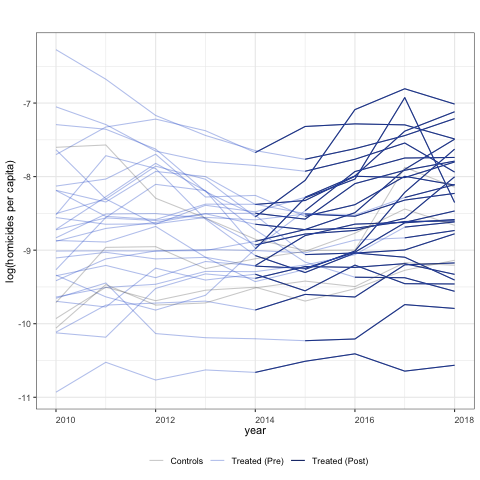
\includegraphics[width=0.55\textwidth]{Figures_pres/reform_treatment_defunciones.png}
       \captionsetup{justification=centering}
          
\hyperlink{why_mexico}{\beamerbutton{Why Mexico?}}
 
\end{figure}    

\end{frame} 
%_____________________________________________________________________
\begin{frame}[label=why_security, noframenumbering]{Why public security?}

\begin{itemize}
	\item Most relevant public good demand in the country since 2007
	       \begin{figure}
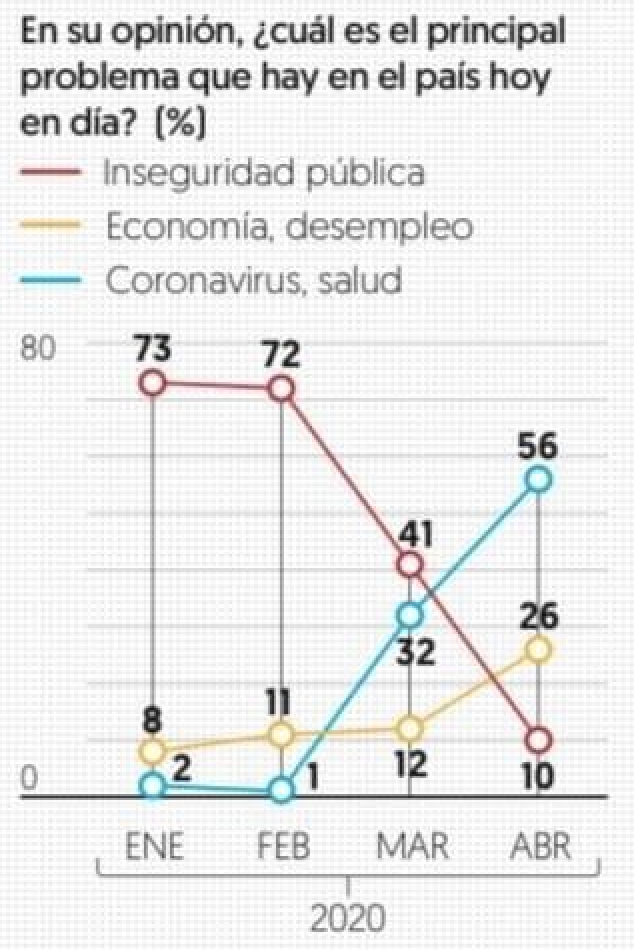
\includegraphics[width=0.3\textwidth]{Figures_pres/leadingproblem_mexico2.png} 
       \captionsetup{justification=centering}
      \end{figure} 
      
	\item No citizen preference variation across the country: help identification
\end{itemize} 
	\hyperlink{this_paper}{\beamerbutton{This Paper}}

\end{frame} 

%_____________________________________________________________________
\begin{frame}[label=reform_background, noframenumbering]{2014 Term Limit Reform: background}
 
\begin{itemize}
	\item Since 1933 constitutional amendment with reelection ban by he PNR (former PRI): control party members
	\item 2012 Felipe Calderon introduced term limit reform to Congress, blocked by the PRI
	\item 2012 Pena Nieto (PRI) won presidency with multiple electoral irregularities
	\item 2013 Pushed set of Energy and Fiscal reforms
	\item Mexican Pact Accord between PRI, PAN and PRD to avoid political gridlocks
	\item Electoral Reform used as a bargaining chip to approve PRI's Energy reform
	\item Faced opposition by governors
	\item President Pena Nieto ``exhorted" local legislator to approve the reform
	\item Promulgated on Jan. 31, 2014

\end{itemize} 
	
	 \hyperlink{reform_content}{\beamerbutton{Reform Content}} 
\end{frame} 
%_____________________________________________________________________
\begin{frame}[label=ihs_results, noframenumbering]{With IHS transformation}
\begin{figure}[h] 
\centering
\caption{Effect of Term Limit Reform of 2014 on Violence, IHS transformation}
\label{fig:event_study_ihs}
   
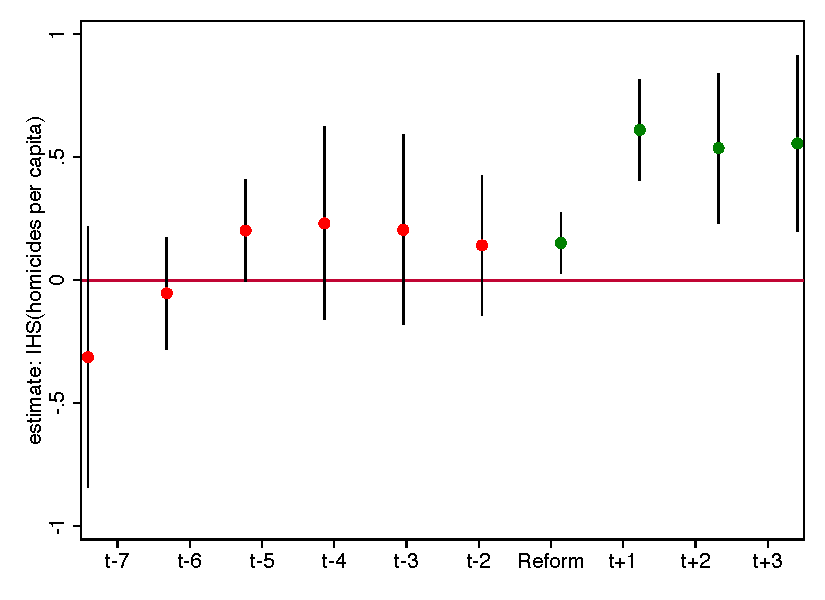
\includegraphics[width=0.65\textwidth]{Figures_pres/event_study_ihs.pdf}
       \captionsetup{justification=centering}
       
 %{\footnotesize Note: IW estimators for each lead and lag relative to the first year of treatment.}  
\hyperlink{main_results}{\beamerbutton{Main Results}}

\end{figure}    

\end{frame} 
%_____________________________________________________________________
\begin{frame}[label=event_by_event, noframenumbering]{Event-by-event analysis}
\begin{itemize}
 		  \setlength\itemsep{1em}   
	\item Estimate treatment effects for each treated Mexican state (28) (\textcolor{blue}{Cengiz et. al, 2019)}
	\item Create sate-event specific panel datasets contain the treated state and all other non yet treated states
	\item Estimate 28 DiD regressions: 

\begin{equation}
y_{mt}=\mu_m	 + \mu_t + \gamma Reform_{mt} + \epsilon_{mt}
\end{equation} 
	%\item $Reform_{mt}$: indicator treatment

	\item \alert{Looking for: no clustering across early and late adopters} 

\end{itemize}
  \hyperlink{identification2}{\beamerbutton{Identification}}  


\end{frame}

%_____________________________________________________________________
\begin{frame}[label=event_by_event_figure, noframenumbering]%{Event-by-event analysis following \textcolor{blue}{Cengiz et. al (2019)}} 
\begin{figure}[H]
\centering
\caption{``Event-by-event analysis'', 95\% confidence intervals} 
\label{fig:CDLZ}
    
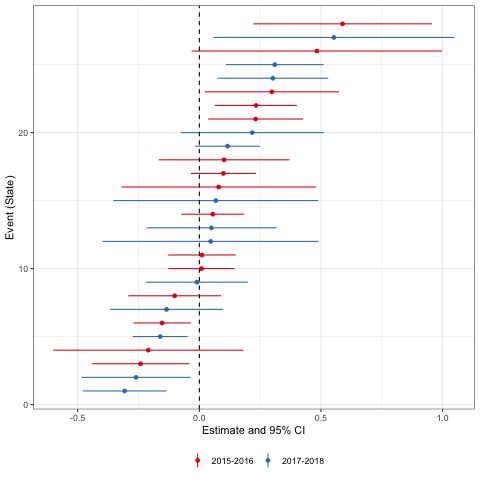
\includegraphics[width=0.55\textwidth]{Figures_pres/CDLZ_cov.png}
       \captionsetup{justification=centering}
 %{\textbf Note:} Estimate separate treatment effects for each event, i.e. each Mexican state in the sample. Each event dataset contains the treated state and all other states that never received treatment or received treatment after the sample window ($t+1$).  
 \\ 
  \hyperlink{stacked_analysis}{\beamerbutton{Stacked dataset analysis}}  
    \hyperlink{identification2}{\beamerbutton{Identification}}  

 
\end{figure}   
 
\end{frame}
%___________
\begin{frame}[label=stacked_analysis, noframenumbering]%{Event-by-event analysis following \textcolor{blue}{Cengiz et. al (2019)}} 
\begin{figure}[H]
\centering
\caption{``Stacked dataset analysis'', 95\% confidence intervals} 
\label{fig:stacked_wcontrols}
      
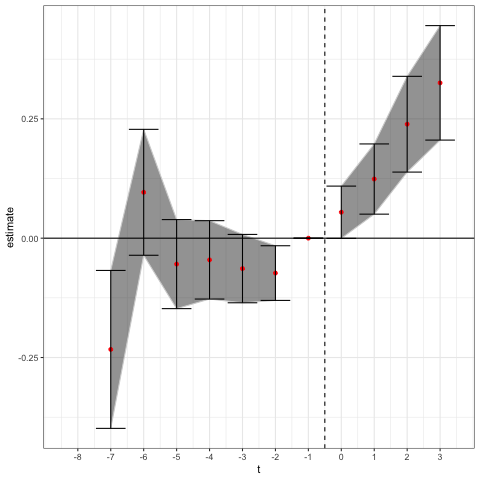
\includegraphics[width=0.55\textwidth]{Figures_pres/stacked_dataset_wcontrols.png}
       \captionsetup{justification=centering}
 %{\textbf Note:} I take each of the ``event-by-event'' datasets from Figure \ref{fig:CDLZ}, stack estimates by cohort and estimate one set of lead and lag variables not using prior treated units as controls..  
 \\ 
  \hyperlink{event_by_event_figure}{\beamerbutton{Event-by-event analysis}}     \hyperlink{identification2}{\beamerbutton{Identification}}   

 
\end{figure}   
 
\end{frame}

%_______________________________________________________
\begin{frame}[label=diff_datasets, noframenumbering]
\begin{table}[htbp]\def\sym#1{\ifmmode^{#1}\else\(^{#1}\)\fi}
\centering  
\caption{Effect of 2014 Term Limit Reform on Violence, using different homicide databases} 
\label{tab:abraham_sun_lagdv_voutcomes}
\scalebox{0.35}{
\begin{tabular}{lcccc}
\hline \hline
\\ \multicolumn{5}{l}{Dependent variable: log(homicides per capita)}\\
\\
Source: & \multicolumn{1}{c}{INEGI} & \multicolumn{3}{c}{SNSP} \\
\cmidrule(lrr){2-2}  \cmidrule(lrr){3-5}\\
&  & \multicolumn{1}{c}{(old measure)} & \multicolumn{1}{c}{(new measure)} & \multicolumn{1}{c}{(combined)}\\
& \multicolumn{1}{c}{(1)} & \multicolumn{1}{c}{(2)} & \multicolumn{1}{c}{(3)} & \multicolumn{1}{c}{(4)} \\
\cmidrule(lrr){2-2} \cmidrule(lrr){3-3}  \cmidrule(lrr){4-4} \cmidrule(lrr){5-5}\\
\addlinespace
Lag 7 years &     $ -0.2569^{} $ &     &  &    \\
&     ($0.1766$) &    &  &  \\
Lag 6 years &     $ -0.0416^{} $ &      &  $ -0.0826^{**} $ &  $ -0.0711^{**} $  \\
&     ($0.0820$) &    & ($0.0381$) & ($0.0343$) \\
Lag 5 years &     $ 0.1505^{*} $ &      &  $ -0.0398^{*} $ &  $ -0.0387^{*} $ \\
&     ($0.0777$) &   & ($0.0210$) & ($0.0198$) \\
Lag 4 years &     $ 0.1534^{} $ &      &   $ 0.0482^{} $ &   $ 0.1170^{} $  \\
&     ($0.1571$) &   & ($0.0769$) & ($0.0776$) \\
Lag 3 years &     $ 0.1274^{} $ &      &   $ -0.0813^{} $ &   $ 0.1105^{} $ \\
&     ($0.1551$) &   & ($0.1318$) & ($0.1524$) \\
Lag 2 years &     $ 0.0873^{} $ &     $ -0.0107^{} $ &  $ -0.0638^{} $  &  $ 0.0766^{} $  \\
&     ($0.1143$) &   ($0.0261$) & ($0.0964$) & ($0.0972$) \\
Reform, time 0 &     $ 0.1080^{**} $ &     $ 0.0130^{} $ &   $ 0.0825^{} $   &   $ 0.1898^{**} $ \\
&     ($0.0518$) &   ($0.0230$) & ($0.0702$) & ($0.0711$) \\
Lead 1 year &     $ 0.4616^{***} $ &     $ 0.0479^{} $ &    $ 0.3014^{***} $ &    $ 0.5458^{***} $ \\
&     ($0.0804$) &   ($0.0335$) & ($0.0921$) & ($0.1258$) \\
Lead 2 years &     $ 0.3939^{***} $ &     $ 0.0490^{**} $ &   $ 0.0782^{} $  &   $ 0.4253^{**} $  \\
&     ($0.1165$) &   ($0.0198$) & ($0.0831$) & ($0.1574$) \\
Lead 3 years &     $ 0.4061^{***} $ &     $ 0.2470^{***} $ &    &   $ 0.5446^{***} $ \\
&     ($0.1386$) &   ($0.0810$) &  & ($0.1589$) \\
\\
\addlinespace
Observations       &              8,592    &              3,088    &           5,452      &           6,515  \\
R-squared        &          0.7776 &          0.8479    &           0.7359       &           0.7312   \\
Mun. FEs      &     \checkmark         &  \checkmark   &     \checkmark         &  \checkmark    \\
Year. FEs    &     \checkmark         &  \checkmark   &     \checkmark         &  \checkmark   \\
State Controls$^b$  &    \checkmark      &       \checkmark  &    \checkmark      &   \checkmark    \\
Cohort weighted  &   \checkmark      &       \checkmark  &   \checkmark       &   \checkmark    \\
Lag DV &    \checkmark    &       \checkmark  &    \checkmark      &   \checkmark    \\
\hline \hline
%\multicolumn{5}{p{0.8\textwidth}}{\footnotesize{Notes: Coefficients show IW estimators following \citet{abraham_sun_2020}. Two relative time periods (lag 8 and 1) are removed to avoid collinearity problems noted by \citet{abraham_sun_2020} in column (1). Missing values correspond to missingness in the data. Standard errors in parentheses are clustered at the state level, with the following significance-level: $^{***}$ 1\%; $^{**}$ 5\%; and $^*$ 10\%, that refer to two-sided t-test with the null hypothesis equal to 0 for each relative time period. $^a$ Refers to the inverse hyperbolic sine transformation. $^b$ State-level controls include governor winning margin in last pre-treatment election and an indicator of whether the governor's party is the same as the federal incumbent party.}} \\
\end{tabular}
}
\end{table}
   \hyperlink{robustness}{\beamerbutton{Robustness}}  

\end{frame} 
%_____________________________________________________________________
\begin{frame}[label=sensitivity_analysis, noframenumbering]
 
 \begin{figure}[!htbp]  
\centering
\caption{Sensitivity Analysis for $\theta=\tau_3$ using $\Delta = \Delta^{SD}(M)$} 
\label{fig:pretrends_sensitivity}
 
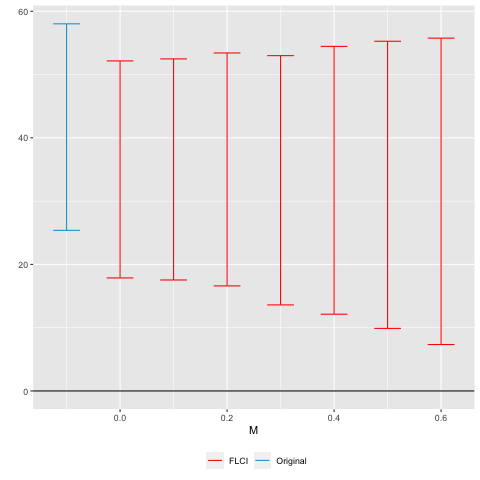
\includegraphics[width=0.5\textwidth]{Figures_pres/pretrends_sensitivity.png}
       \captionsetup{justification=centering}
\bigskip   
 
{\footnotesize Note: $M$ lower bound=0; $M$ upper bound=0.5536. Blue confidence interval shows the third lag after treatment.} 
 \\  
  \hyperlink{robustness}{\beamerbutton{Robustness}}  
\end{figure} 
\end{frame}

%_____________________________________________________________________
\begin{frame}[label=sensitivity_negative, noframenumbering]
 
\begin{figure}[h]  
\centering
\caption{Monotonically decreasing pre-trend violation}% using $\Delta = \Delta^{SDD}(M)$} 
%\label{fig:pretrend_violations} 

\begin{center} 
	%{\textbf Figure A: Monotonically decreasing pre-trend violation} 
\end{center} 
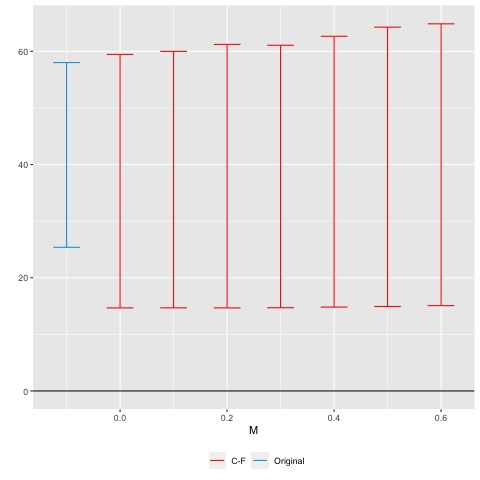
\includegraphics[width=0.45\textwidth]{Figures_pres/pretrends_sensitivity_decreasing.png}

       \\  
{\footnotesize Note: $M$ lower bound=0; $M$ upper bound=0.5536. Blue confidence interval shows the third lag after treatment.} 
 \\  
  \hyperlink{robustness}{\beamerbutton{Robustness}} 
\end{figure} 
      
\end{frame}
%_____________________________________________________________________
\begin{frame}[label=sensitivity_positive, noframenumbering]
 
\begin{figure}[h]  
\centering
\caption{Monotonically increasing pre-trend violation}% using $\Delta = \Delta^{SDD}(M)$} 
%\label{fig:pretrend_violations} 

\begin{center} 
	%{\textbf Figure A: Monotonically decreasing pre-trend violation} 
\end{center} 
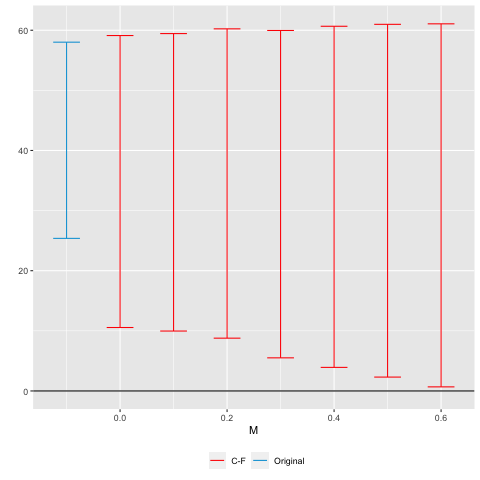
\includegraphics[width=0.45\textwidth]{Figures_pres/pretrends_sensitivity_increasing.png}

       \\   
{\footnotesize Note: $M$ lower bound=0; $M$ upper bound=0.5536. Blue confidence interval shows the third lag after treatment.} 
 \\  
  \hyperlink{robustness}{\beamerbutton{Robustness}} 
\end{figure} 
      
\end{frame}

%_____________________________________________________________________
\begin{frame}[label=falsification, noframenumbering]
 
 \begin{figure}[h]  
\centering
\caption{Falsifying Term-Limit Reform Treatment Assignment, post-treatment periods} 
\label{fig:falsification}
  
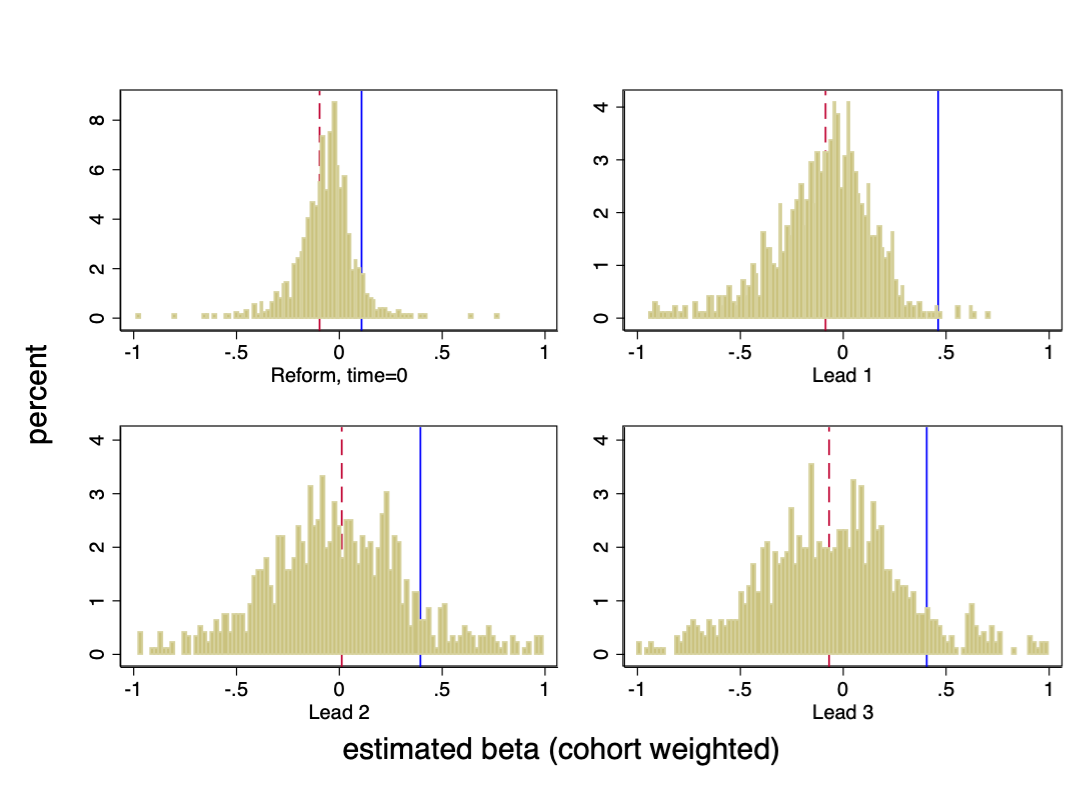
\includegraphics[width=0.75\textwidth]{Figures_pres/falsification_post.png}
       \captionsetup{justification=centering}
       \\  
  %{\textbf Note: Estimated (cohort weighted) beta coefficients distribution of 1,000 simulations following equation \ref{eq:abraham}. For each simulation I carry a random Bernoulli draw with success rate equal to the proportion of treated states by the Electoral Reform by time period. Blue line displays the estimated effect of the electoral reform on logged homicides per capita of column (2) o Table \ref{tab:abraham_sun_lagdv}. Red line shows the average estimated effect of the simulations.}     
 
  \hyperlink{robustness}{\beamerbutton{Robustness}} 
\end{figure} 
      
\end{frame}
%_____________________________________________________________________
\begin{frame}[label=mando_unico, noframenumbering]
 
\begin{figure}[h]  
\centering
\caption{Effect of Term Limit Reform on Violence, by security cooperation agreement} 
\label{fig:split_mando_unico}
  
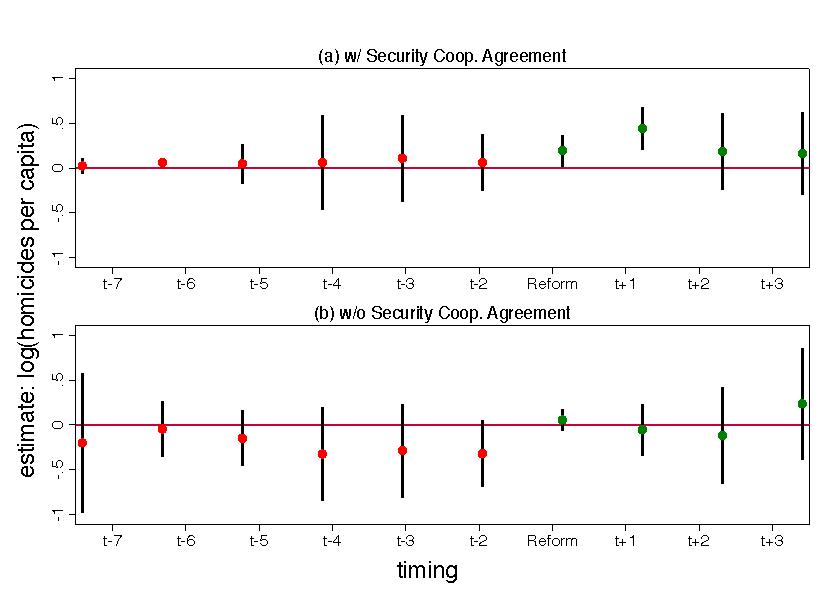
\includegraphics[width=0.75\textwidth]{Figures_pres/event_study_wacuerdo2_placebo.pdf}
    
 %{\textbf Note: Estimates of Figure (a) and (b) correspond to those of Appendix Table \ref{tab:abraham_sun_lagdv_splitmandounico}. Figure (a) includes those municipalities with a security cooperation agreement with upper administrative units, i.e. the state or central government. Figure (b) includes those municipalities without any security cooperation agreement.} 
  \hyperlink{robustness}{\beamerbutton{Robustness}} 
\end{figure} 
      
\end{frame} 

%--------------
\begin{frame}[label=mando_unico_control, noframenumbering]
  
\begin{table}[htbp]\def\sym#1{\ifmmode^{#1}\else\(^{#1}\)\fi}
\centering
\caption{Effect of 2014 Term Limit Reform on Violence, controlling for security cooperation agreements}
\label{tab:abraham_sun_lagdv_mandounico}
\scalebox{0.4}{
\begin{tabular}{lcc}
\hline \hline
\\ \multicolumn{3}{l}{Dependent variable:}\\
& \multicolumn{1}{c}{log(homicide per capita)} & \multicolumn{1}{c}{ihs(homicide per capita)$^{a}$} \\
& \multicolumn{1}{c}{(1)} & \multicolumn{1}{c}{(2)} \\
\cmidrule(lrr){2-2}  \cmidrule(lrr){3-3}\\
\addlinespace
Lag 7 years &      $ -0.2675^{} $ &  $ -0.3293^{} $   \\
& ($ 0.1675$) & ($ 0.2478 $) \\
Lag 6 years &          $ -0.0463^{} $ &   $ -0.0607^{} $  \\
& ($ 0.0789$) & ($ 0.1071 $) \\
Lag 5 years &        $ 0.1419^{*} $ &   $ 0.1893^{*} $ \\
& ($ 0.0793$) & ($ 0.1034 $) \\
Lag 4 years &         $ 0.1367^{} $ &      $ 0.2069^{} $  \\
& ($ 0.1565$) & ($ 0.1913 $) \\
Lag 3 years &        $ 0.1132^{} $ &     $ 0.1833^{} $ \\
& ($ 0.1544$) & ($ 0.1887 $) \\
Lag 2 years &        $ 0.0785^{} $ &    $ 0.1282^{} $  \\
& ($ 0.1139$) & ($ 0.1887 $) \\
Reform, time 0 &        $ 0.1045^{**} $ &     $ 0.1472^{**} $ \\
& ($ 0.0506$) & ($ 0.0600 $) \\
Lead 1 year &         $ 0.4623^{***} $ &       $ 0.6120^{***} $ \\
& ($ 0.0783$) & ($ 0.0975 $) \\
Lead 2 years &         $ 0.3721^{***} $ &      $ 0.5068^{***} $  \\
& ($ 0.1132$) & ($ 0.1456 $) \\
Lead 3 years &        $ 0.3938^{***} $ &     $ 0.5380^{***} $ \\
& ($ 0.1355$) & ($ 0.1713 $) \\
\addlinespace
Observations       &                  8,442        &           8,442  \\
R-squared        &              0.7786        &           0.7035   \\
Mun. FEs       &     \checkmark         &  \checkmark    \\
Year. FEs       &     \checkmark         &  \checkmark   \\
State Controls$^b$   &    \checkmark      &   \checkmark    \\
Cohort weighted   &   \checkmark       &   \checkmark    \\
Lag DV &          \checkmark         &   \checkmark    \\
Security Coop. Agreement &          \checkmark         &   \checkmark    \\
\hline \hline
%\multicolumn{3}{p{0.9\textwidth}}{\footnotesize{Notes: Coefficients show IW estimators following \citet{abraham_sun_2020}. Two relative time periods (lag 8 and 1) are removed to avoid collinearity problems noted by \citet{abraham_sun_2020}. Standard errors in parentheses are clustered at the state level, with the following significance-level: $^{***}$ 1\%; $^{**}$ 5\%; and $^*$ 10\%, that refer to two-sided t-test with the null hypothesis equal to 0 for each relative time period. $^a$ Refers to the inverse hyperbolic sine transformation. $^b$ State-level controls include governor winning margin in last pre-treatment election and an indicator of whether the governor's party is the same as the federal incumbent party.}} \\
\end{tabular}
}
\end{table}


	\hyperlink{robustness}{\beamerbutton{Robustness}} 
	
\end{frame}
%______________
\begin{frame}[label=event_by_event_figure2, noframenumbering]%{Event-by-event analysis following \textcolor{blue}{Cengiz et. al (2019)}} 
\begin{figure}[H]
\centering
\caption{``Event-by-event analysis'', 95\% confidence intervals} 
\label{fig:CDLZ}
    
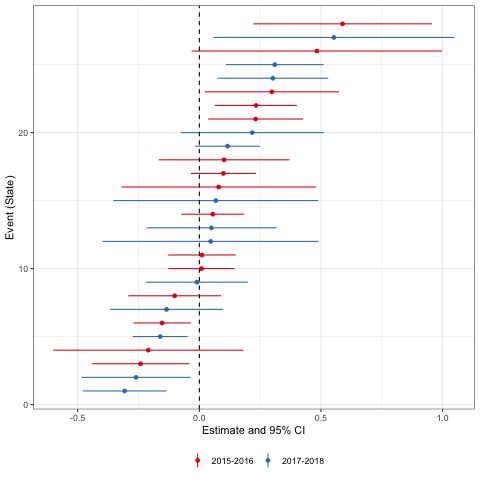
\includegraphics[width=0.6\textwidth]{Figures_pres/CDLZ_cov.png}
       \captionsetup{justification=centering}
 %{\textbf Note:} Estimate separate treatment effects for each event, i.e. each Mexican state in the sample. Each event dataset contains the treated state and all other states that never received treatment or received treatment after the sample window ($t+1$).  
 \\ 
  \hyperlink{mechanism_identification}{\beamerbutton{Mechanism: identification}}  
 
\end{figure}   
 
\end{frame}

%_____________________________________________________________________
\begin{frame}[label=population, noframenumbering]{No discontinuous jump of population}
\begin{figure}[h] 
\centering 
\caption{Effect of Term Limit Reform of 2014 on Population, IW estimators with 95\% confidence intervals}
\label{fig:incumbency_adv_1234}
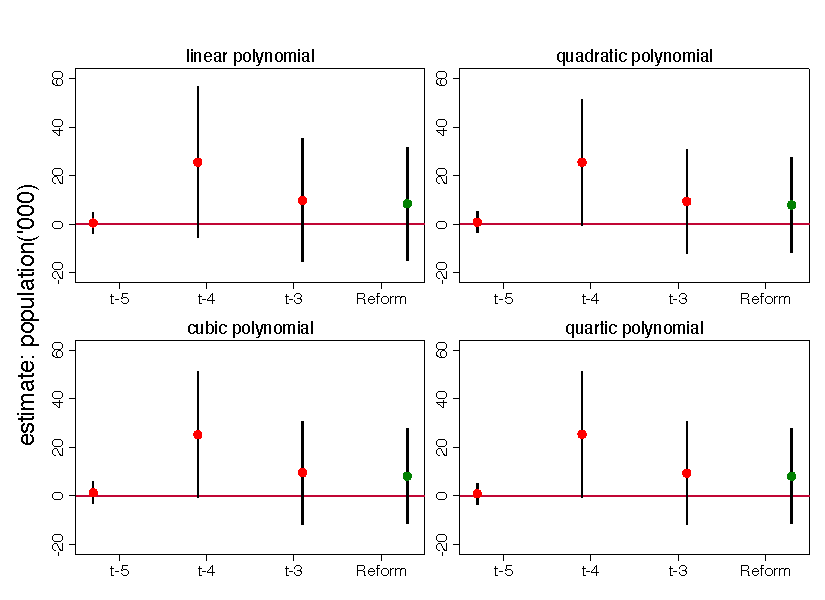
\includegraphics[width=0.65\textwidth]{Figures_pres/pop.pdf}
       \captionsetup{justification=centering}

 %{\footnotesize Note: IW estimators for each lead and lag relative to the first year of treatment.} 
  \hyperlink{mechanism_identification}{\beamerbutton{Mechanism: identification}} 

\end{figure} 
\end{frame}
%___________
\begin{frame}[label=mccrary_test, noframenumbering]
 
\begin{figure}[H]
\centering
\caption{McCrary Test, quadratic polynomial}
  \label{fig:mccrary}
 
 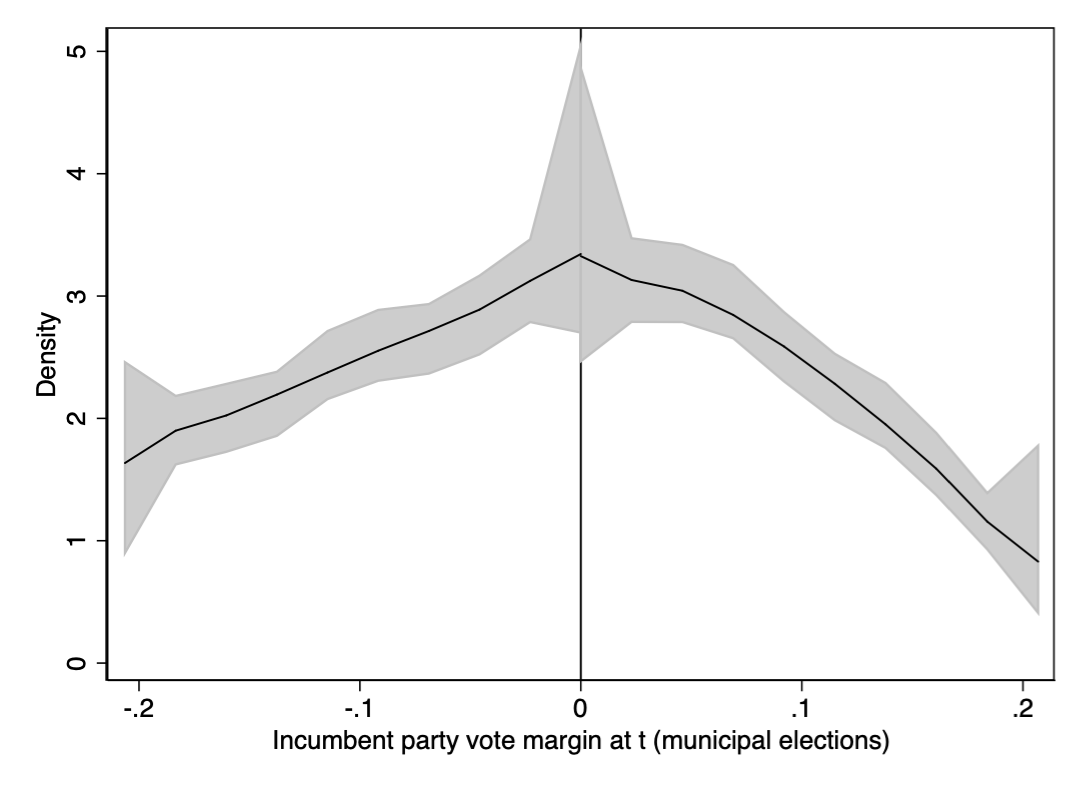
\includegraphics[width=0.7\textwidth]{Figures_pres/mccrary_test_pol2.png}
       \captionsetup{justification=centering}
 %{\textbf Note: .}      
  
  \hyperlink{mechanism_identification}{\beamerbutton{Mechanism: identification}}
\end{figure} 
      
\end{frame}
%----------------------------------------------
\begin{frame}[label=rdd_figure, noframenumbering]

\begin{figure}[H]
\centering
\caption{Effect of Term Limit Reform of 2014 on Incumbency Advantage, quadratic polynomial}
  \label{fig:incumbency_advantage} 

	%{\textbf Figure A: quadratic polynomial}
 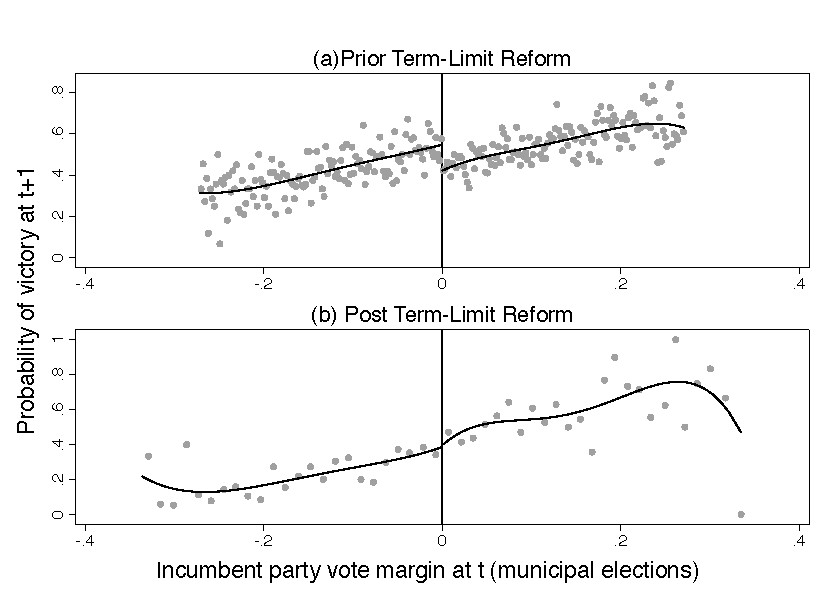
\includegraphics[width=0.7\textwidth]{Figures_pres/RDD_incumbency_pol2.pdf}
     \captionsetup{justification=centering}  
        
\end{figure}  
\hyperlink{mechanism_identification}{\beamerbutton{Mechanism: identification}}  

	
\end{frame}

%----------------------------------------------
\begin{frame}[label=rdd_table, noframenumbering]  

\begin{table}[!htbp]\def\sym#1{\ifmmode^{#1}\else\(^{#1}\)\fi}
\caption{Regression Discontinuity Design of Close Elections on Incumbency Advantage, comparing pre and post-Term Limit Reform estimates}
\label{tab:rdd}  
\begin{center} 
\scalebox{0.55}{
\begin{tabular}{lcccccccc}
  
\hline \hline   
\\
    
\multicolumn{9}{l}{Dependent variable:}\\
  
            &\multicolumn{2}{c}{linear polynomial}      &\multicolumn{2}{c}{quadratic polynomial}   &\multicolumn{2}{c}{cubic polynomical}      &\multicolumn{2}{c}{quartic polynomial}     \\\cmidrule(lr){2-3}\cmidrule(lr){4-5}\cmidrule(lr){6-7}\cmidrule(lr){8-9}
            &\multicolumn{1}{c}{(1)}         &\multicolumn{1}{c}{(2)}         &\multicolumn{1}{c}{(3)}         &\multicolumn{1}{c}{(4)}         &\multicolumn{1}{c}{(5)}         &\multicolumn{1}{c}{(6)}         &\multicolumn{1}{c}{(7)}         &\multicolumn{1}{c}{(8)}         \\
\addlinespace
Probability of victory at t+1$^a$&     -0.1075\sym{***}&      0.0750         &     -0.1114\sym{***}&      0.0595         &     -0.1130\sym{***}&      0.0639         &     -0.1132\sym{***}&      0.0565         \\
            &    (0.0217)         &    (0.0636)         &    (0.0274)         &    (0.0846)         &    (0.0330)         &    (0.0925)         &    (0.0387)         &    (0.1182)         \\
\addlinespace
Observations&       8,623         &         890         &      10,138         &         955         &      10,849         &       1,116         &      11,262         &       1,064         \\
Post Reform (2014)&                     &  \checkmark         &                     &  \checkmark         &                     &  \checkmark         &                     &  \checkmark         \\
 

             
\hline \hline   
\end{tabular}         
}
\end{center} 
\end{table} 
\hyperlink{mechanism_identification}{\beamerbutton{Mechanism: identification}} 

	
\end{frame}
%_____________________________________________________________________
\begin{frame}[label=strategic1, noframenumbering]{Strategic placement of effort: party alignment}
 
\begin{table}[htbp]\def\sym#1{\ifmmode^{#1}\else\(^{#1}\)\fi}
\centering
\caption{Total Interaction Effect:$^a$ the role of Alignment with Federal Government and Municipal Winning Margin}
\label{tab:abraham_sun_heteffects}
\scalebox{0.6}{
\begin{tabular}{lcccc}
\hline \hline
\\ \multicolumn{5}{l}{Dependent variable:}\\
& \multicolumn{2}{c}{log(homicide per capita)} & \multicolumn{2}{c}{ihs(homicide per capita)$^{b}$} \\
& \multicolumn{1}{c}{(1)} & \multicolumn{1}{c}{(2)} & \multicolumn{1}{c}{(3)} & \multicolumn{1}{c}{(4)} \\
\cmidrule(lrr){2-3}  \cmidrule(lrr){4-5}\\
\addlinespace
Reform (t+3)*Alignment Fed. Gov. &     $ -0.1397^{*} $ &  &  $ -0.1748^{**} $  & \\
&     ($ 0.0690 $) &  & ($ 0.0816 $)  & \\
Reform (t+3)*Winning Margin &    &   $ -0.3325^{} $ &  &  $ -0.4745^{} $ \\
&    &     ($ 0.4494 $) & & ($ 0.5430 $)  \\
\\
\addlinespace
Observations       &              2,966    &              2,966    &           2,966      &           2,966  \\
R-squared       &        0.8244    &        0.7759    &     0.8234      &     0.7748  \\
Mun. FEs      &     \checkmark         &  \checkmark   &     \checkmark         &  \checkmark    \\
Year. FEs    &     \checkmark         &  \checkmark   &     \checkmark         &  \checkmark   \\
State Controls$^c$  &  \checkmark       &       \checkmark  &  \checkmark        &   \checkmark    \\
Cohort weighted$^d$  &   \checkmark      &       \checkmark  &   \checkmark       &   \checkmark    \\
\hline \hline
%\multicolumn{5}{p{1\textwidth}}{\footnotesize{Notes:$^a$ Total interaction effect tests the linear hypothesis of the estimated coefficient of alignment with Federal Government indicator (winning margin) + estimated coefficient of the interaction of alignment (winning margin)*lead t=3. This is a post-estimation test using the same specification as that of Table \ref{tab:abraham_sun_lagdv} column (1). Other leads and the indicator at time t=0 when reform came to effect are omitted due to collinearity. Standard errors of linear hypothesis test in parentheses with the following significance-level: $^{***}$ 1\%; $^{**}$ 5\%; and $^*$ 10\%, that refer to two-sided test with the null hypothesis equal to 0. Main regression with standard errors clustered at the state-level. $^b$ Refers to the inverse hyperbolic sine transformation. $^c$ State-level controls include governor winning margin in last pre-treatment election and an indicator of whether the governor's party is the same as the federal incumbent party. I also include the lag of the outcome, i.e. logged homicides per capita as control. $^d$ Estimates weighted by each cohort's relative share of the sample following \citet{abraham_sun_2020}.}} \\
\end{tabular}
}
\end{table}
\hyperlink{effort}{\beamerbutton{Effort}} 


\end{frame}

%_____________________________________________________________________
\begin{frame}[label=strategic2, noframenumbering]{Strategic placement of effort: ``not in my backyard"} 
\begin{table}[htbp]\def\sym#1{\ifmmode^{#1}\else\(^{#1}\)\fi}
\centering
\caption{Total Interaction Effect of Partisanship on Public Security Effort$^a$}
\label{tab:abraham_sun_pri_effort}
\scalebox{0.6}{
\begin{tabular}{lcccc}
\hline \hline
\\ \multicolumn{5}{l}{Dependent variable:}\\
& \multicolumn{2}{c}{log(cocaine)$^b$} & \multicolumn{2}{c}{log(heroine)$^b$} \\
& \multicolumn{1}{c}{(1)} & \multicolumn{1}{c}{(2)} & \multicolumn{1}{c}{(3)} & \multicolumn{1}{c}{(4)} \\
\cmidrule(lrr){2-3}  \cmidrule(lrr){4-5}\\
\addlinespace
Reform (t+3)*PRI &     $ 0.0616^{} $ &  &  $ -0.0295^{} $  & \\
&     ($ 0.0561 $) &  & ($ 0.0429 $)  & \\
Reform (t+3)*PAN &    &   $ 0.1004^{**} $ &  &  $ 0.0267^{*} $ \\
&    &     ($ 0.0443 $) & & ($ 0.0147 $)  \\
\\
\addlinespace
Observations       &              4,550    &              4,550    &           4,550      &           4,550  \\
R-squared       &        0.4533    &        0.4537    &     0.3372      &     0.3373  \\
Mun. FEs      &     \checkmark         &  \checkmark   &     \checkmark         &  \checkmark    \\
Year. FEs    &     \checkmark         &  \checkmark   &     \checkmark         &  \checkmark   \\
State Controls$^c$  &  \checkmark       &       \checkmark  &  \checkmark        &   \checkmark    \\
Cohort weighted$^d$  &   \checkmark      &       \checkmark  &   \checkmark       &   \checkmark    \\
\hline \hline
%\multicolumn{5}{p{0.65\textwidth}}{\footnotesize{Notes:$^a$ Total interaction effect tests the linear hypothesis of the estimated coefficient of PRI mayor (PAN mayor) + estimated coefficient of the interaction of PRI (PAN)*lead t=3. This is a post-estimation test using the same specification as that of Table \ref{tab:abraham_sun_lagdv} column (1). Other leads and the indicator at time t=0 when reform came to effect are omitted due to collinearity. Standard errors of linear hypothesis test in parentheses with the following significance-level: $^{***}$ 1\%; $^{**}$ 5\%; and $^*$ 10\%, that refer to two-sided test with the null hypothesis equal to 0. Main regression with standard errors clustered at the state-level. $^b$ Refers to the inverse hyperbolic sine transformation. $^c$ State-level controls include governor winning margin in last pre-treatment election and an indicator of whether the governor's party is the same as the federal incumbent party. I also include the lag of the outcome, i.e. logged homicides per capita as control. $^d$ Estimates weighted by each cohort's relative share of the sample following \citet{abraham_sun_2020}.}} \\
\end{tabular}
}
\end{table}
\hyperlink{effort}{\beamerbutton{Effort}} 

\end{frame}

%_____________________________________________________________________
\begin{frame}[label=strategic3, noframenumbering]{Strategic placement of effort: ``let others burn"} 
\begin{table}[htbp]\def\sym#1{\ifmmode^{#1}\else\(^{#1}\)\fi}
\centering 
\caption{Total Interaction Effect of Partisanship on Violence$^a$}
\label{tab:abraham_sun_pri}
\scalebox{0.6}{
\begin{tabular}{lcccc}
\hline \hline
\\ \multicolumn{5}{l}{Dependent variable:}\\
& \multicolumn{2}{c}{log(homicide per capita)} & \multicolumn{2}{c}{ihs(homicide per capita)$^{b}$} \\
& \multicolumn{1}{c}{(1)} & \multicolumn{1}{c}{(2)} & \multicolumn{1}{c}{(3)} & \multicolumn{1}{c}{(4)} \\
\cmidrule(lrr){2-3}  \cmidrule(lrr){4-5}\\
\addlinespace
Reform (t+3)*PRI &     $ -0.0920^{} $ &  &  $ -0.0979^{} $  & \\
&     ($ 0.0759 $) &  & ($ 0.0959 $)  & \\
Reform (t+3)*PAN &    &   $ 0.1444^{*} $ &  &  $ 0.1744^{**} $ \\
&    &     ($ 0.0733 $) & & ($ 0.0842 $)  \\
\\
\addlinespace
Observations       &              2,966    &              2,966    &           2,966      &           2,966  \\
R-squared       &        0.8244    &        0.7759    &     0.8234      &     0.7748  \\
Mun. FEs      &     \checkmark         &  \checkmark   &     \checkmark         &  \checkmark    \\
Year. FEs    &     \checkmark         &  \checkmark   &     \checkmark         &  \checkmark   \\
State Controls$^c$  &  \checkmark       &       \checkmark  &  \checkmark        &   \checkmark    \\
Cohort weighted$^d$  &   \checkmark      &       \checkmark  &   \checkmark       &   \checkmark    \\
\hline \hline
%\multicolumn{5}{p{0.8\textwidth}}{\footnotesize{Notes:$^a$ Total interaction effect tests the linear hypothesis of the estimated coefficient of PRI mayor (PAN mayor) + estimated coefficient of the interaction of PRI (PAN)*lead t=3. This is a post-estimation test using the same specification as that of Table \ref{tab:abraham_sun_lagdv} column (1). Other leads and the indicator at time t=0 when reform came to effect are omitted due to collinearity. Standard errors of linear hypothesis test in parentheses with the following significance-level: $^{***}$ 1\%; $^{**}$ 5\%; and $^*$ 10\%, that refer to two-sided test with the null hypothesis equal to 0. Main regression with standard errors clustered at the state-level. $^b$ Refers to the inverse hyperbolic sine transformation. $^c$ State-level controls include governor winning margin in last pre-treatment election and an indicator of whether the governor's party is the same as the federal incumbent party. I also include the lag of the outcome, i.e. logged homicides per capita as control. $^d$ Estimates weighted by each cohort's relative share of the sample following \citet{abraham_sun_2020}.}} \\
\end{tabular}
}
\end{table}
\hyperlink{effort}{\beamerbutton{Effort}} 


\end{frame} 

%-----------------------------------------------
\begin{frame}[label=quality, noframenumbering]

\begin{table}[htbp]\def\sym#1{\ifmmode^{#1}\else\(^{#1}\)\fi}
\centering
\caption{Event-in-Discontinuity in close elections model: Effect of 2014 Term Limit Reform on Incumbent's Quality }
\label{tab:incumbency_quality}
\scalebox{0.6}{
\begin{tabular}{lcc}
\hline \hline
\\ \multicolumn{3}{l}{Dependent variable:}\\
& \multicolumn{2}{c}{Incumbent quality indicator}   \\
& (1) & (2) \\
& \multicolumn{2}{c}{quadratic polynomial} \\
\cmidrule(lrr){2-3} \\
Lag 6 years &    &     $ -0.2795^{} $  \\
&      &    ($0.5702$)  \\
Lag 5 years &     $ -0.4390^{} $ &       $ -0.0755^{} $  \\
&     ($0.3773$) &    ($0.7316$)  \\
Lag 4 years &     $ -0.3998^{} $ &       $ -2.0649^{***} $\\
&     ($0.6689$) &    ($0.1457$)  \\
Lag 3 years &     $ -0.0573^{} $  &     $ -0.4221^{*} $ \\
&     ($0.6061$) &    ($0.2179$)  \\
Reform, time 0 &    $ 0.4450^{} $ &     $ 0.0584^{} $\\
&     ($0.5035$) &    ($0.0452$)  \\
\\
Observations        &              1,813    &              1,985 \\
R-squared        &          0.7031  &          0.6816 \\
Sample Inc. Adv. DV & Inc. at t-1 won at t+1 & Inc. at t won at t+1 \\
 
\\
 \hline 
\end{tabular}
}
\end{table}

  \hyperlink{alternative_explanations}{\beamerbutton{Alternative Explanations}} 
	
\end{frame}

%------------------------------------------------
\begin{frame}[label=citizens_preferences, noframenumbering]
\begin{table}[htbp]\def\sym#1{\ifmmode^{#1}\else\(^{#1}\)\fi}
\centering   
\caption{Effect of 2014 Term Limit Reform on Violence, controlling for citizens security perception}
\label{tab:abraham_sun_citizensdemands}
\scalebox{0.4}{
\begin{tabular}{lcccc}
\hline \hline
\\ \multicolumn{5}{l}{Dependent variable:}\\
& \multicolumn{2}{c}{log(homicide per capita)} & \multicolumn{2}{c}{ihs(homicide per capita)$^{a}$} \\
& \multicolumn{1}{c}{(1)} & \multicolumn{1}{c}{(2)} & \multicolumn{1}{c}{(3)} & \multicolumn{1}{c}{(4)} \\
\cmidrule(lrr){2-3}  \cmidrule(lrr){4-5}\\
\addlinespace
Lag 7 years &     $ -0.2569^{} $ &      & $ -0.3129^{} $ &   \\
&     ($0.1766$) &    & ($0.2584$) & \\
Lag 6 years &     $ -0.0416^{} $ &  $ -0.0111^{} $    &  $ -0.0535^{} $ &  $ -0.0053^{} $  \\
&     ($0.0820$) &   ($0.0580$) & ($0.1108$) & ($0.0748$) \\
Lag 5 years &     $ 0.1505^{*} $ &   $ -0.0072^{} $   &  $ 0.2019^{*} $ &  $ -0.0056^{} $ \\
&     ($0.0777$) &   ($0.0198$) & ($0.1011$) & ($0.0248$) \\
Lag 4 years &     $ 0.1534^{} $ &   $ 0.0469^{} $   &   $ 0.2315^{} $ &   $ 0.0704^{} $  \\
&     ($0.1571$) &   ($0.0801$) & ($0.1910$) & ($0.0967$) \\
Lag 3 years &     $ 0.1274^{} $ &   $ 0.3133^{} $   &   $ 0.2044^{} $ &   $ 0.4325^{*} $ \\
&     ($0.1551$) &   ($0.2082$) & ($0.1883$) & ($0.2407$) \\
Lag 2 years &     $ 0.0873^{} $ &     $ 0.1054^{} $ &  $ 0.1416^{} $  &  $ 0.1534^{} $  \\
&     ($0.1143$) &   ($0.1362$) & ($0.1386$) & ($0.1608$) \\
Reform, time 0 &     $ 0.1080^{**} $ &     $ 0.1477^{*} $ &   $ 0.1512^{**} $   &   $ 0.1978^{**} $ \\
&     ($0.0518$) &   ($0.0775$) & ($0.0610$) & ($0.0926$) \\
Lead 1 year &     $ 0.4616^{***} $ &     $ 0.2641^{**} $ &    $ 0.6111^{***} $ &    $ 0.3507^{***} $ \\
&     ($0.0804$) &   ($0.1038$) & ($0.0994$) & ($0.1176$) \\
Lead 2 years &     $ 0.3939^{***} $ &     $ 0.1894^{*} $ &   $ 0.5372^{***} $  &   $ 0.2686^{**} $  \\
&     ($0.1165$) &   ($0.0937$) & ($0.1485$) & ($0.1060$) \\
Lead 3 years &     $ 0.4061^{***} $ &     $ 0.2188^{*} $ &   $ 0.5564^{***} $ &   $ 0.3107^{**} $ \\
&     ($0.1386$) &   ($0.1068$) & ($0.1740$) & ($0.1261$) \\
\\
\addlinespace
Observations       &              8,592    &              7,574    &           8,592      &           7,574  \\
R-squared        &          0.7776 &          0.7889    &           0.7025       &           0.7164   \\
Mun. FEs      &     \checkmark         &  \checkmark   &     \checkmark         &  \checkmark    \\
Year. FEs    &     \checkmark         &  \checkmark   &     \checkmark         &  \checkmark   \\
State Controls$^b$  &    \checkmark      &       \checkmark  &    \checkmark      &   \checkmark    \\
Cohort weighted  &   \checkmark      &       \checkmark  &   \checkmark       &   \checkmark    \\
Lag DV &  \checkmark      &       \checkmark  &    \checkmark      &   \checkmark    \\
Citizens' Security Perception$^c$ &    &   \checkmark  &         &   \checkmark    \\
\hline \hline
%\multicolumn{5}{p{0.9\textwidth}}{\footnotesize{Notes: Coefficients show IW estimators following \citet{abraham_sun_2020}. Two relative time periods (lag 8 and 1) are removed to avoid collinearity problems noted by \citet{abraham_sun_2020}; lag 7 is removed in columns (2) and (4) due to collinearity. Standard errors in parentheses are clustered at the state level, with the following significance-level: $^{***}$ 1\%; $^{**}$ 5\%; and $^*$ 10\%, that refer to two-sided t-test with the null hypothesis equal to 0 for each relative time period. $^a$ Refers to the inverse hyperbolic sine transformation. $^b$ State-level controls include governor winning margin in last pre-treatment election and an indicator of whether the governor's party is the same as the federal incumbent party. $^c$ Citizens' Security Perception are state-level covariates that include the percentage of citizens who see narcotraffick as the most worrisome issue in the country, the percentage of citizens who see a lack of punishment of criminals as the most worrisome public issue, the amount of money (in thousands) spend to protect from crime, and citizens trust on local police forces and the army.}} \\
\end{tabular}
}
\end{table}
  \hyperlink{alternative_explanations}{\beamerbutton{Alternative Explanations}} 

	
\end{frame}
 
%_____________________________________________________________________
\begin{frame}[label=citizens_preferences_log, noframenumbering]

\begin{figure}[H]
\centering
\caption{Effect of Term Limit Reform of 2014 on Violence, controlling for citizens' security preferences}
  \label{fig:citizens_preferences_log} 

 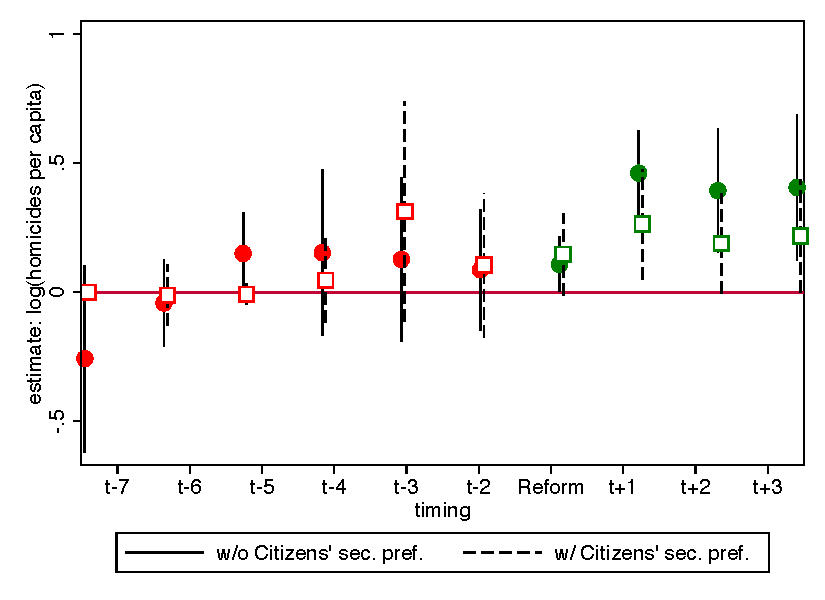
\includegraphics[width=0.7\textwidth]{Figures_pres/citizens_preferences_log.pdf}
     \captionsetup{justification=centering}  
        
\end{figure}  
  \hyperlink{alternative_explanations}{\beamerbutton{Alternative Explanations}} 


\end{frame}

%_____________________________________________________________________
\begin{frame}[label=citizens_preferences_ihs, noframenumbering]
\begin{figure}[H]
\centering
\caption{Effect of Term Limit Reform of 2014 on Violence, controlling for citizens' security preferences}
  \label{fig:citizens_preferences_ihs} 

 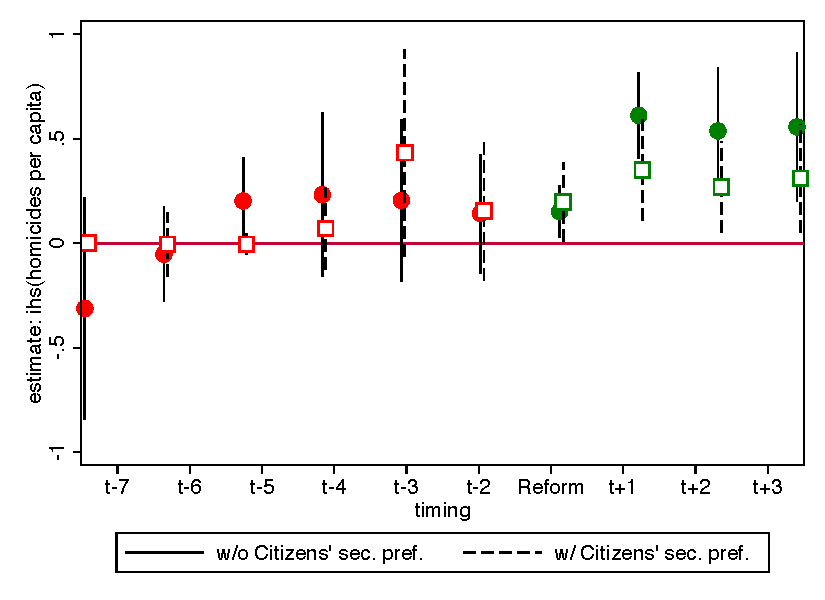
\includegraphics[width=0.7\textwidth]{Figures_pres/citizens_preferences_ihs.pdf}
     \captionsetup{justification=centering}  
        
\end{figure}  
  \hyperlink{alternative_explanations}{\beamerbutton{Alternative Explanations}} 

\end{frame}
   
   
%_____________________________________________________________________
\begin{frame}[label=capture,noframenumbering] 

\begin{table}[htbp]\def\sym#1{\ifmmode^{#1}\else\(^{#1}\)\fi}  
\centering  
\caption{Total Interaction Effect of Term Limit Reform and Drug Trafficking Organization Presence on Violence$^a$}
\label{tab:abraham_sun_dto_het}
\scalebox{0.65}{
\begin{tabular}{lcccc}
\hline \hline
\\ \multicolumn{5}{l}{Dependent variable:}\\
& \multicolumn{2}{c}{log(homicide per capita)} & \multicolumn{2}{c}{ihs(homicide per capita)$^{b}$} \\
& \multicolumn{1}{c}{(1)} & \multicolumn{1}{c}{(2)} & \multicolumn{1}{c}{(3)} & \multicolumn{1}{c}{(4)} \\
\cmidrule(lrr){2-3}  \cmidrule(lrr){4-5}\\
\addlinespace
Reform (t+3) X Proximity to U.S.  &     $ -0.3094^{**} $ &  &  $ -0.3761^{**} $  & \\
&     ($ 0.1210 $) &  & ($ 0.1539 $)  & \\
Reform (t+3) X Cartel presence (indicator) &    &   $ 0.1412^{**} $ &  &  $ 0.1398^{*} $ \\
&    &     ($ 0.0670 $) & & ($ 0.0818 $)  \\
\addlinespace
Observations       &              8,592    &              8,592    &           8,592      &           8,592  \\
R-squared       &        0.7779    &        0.7030    &     0.7778      &     0.7027  \\
Mun. FEs      &     \checkmark         &  \checkmark   &     \checkmark         &  \checkmark    \\
Year. FEs    &     \checkmark         &  \checkmark   &     \checkmark         &  \checkmark   \\
State Controls$^c$  &  \checkmark       &       \checkmark  &  \checkmark        &   \checkmark    \\
Cohort weighted$^d$  &   \checkmark      &       \checkmark  &   \checkmark       &   \checkmark    \\
Lag DV &  \checkmark      &       \checkmark  &    \checkmark      &   \checkmark    \\
\hline \hline
%\multicolumn{5}{p{1.1\textwidth}}{\footnotesize{Notes:$^a$ Total interaction effect tests the linear hypothesis of the estimated coefficient of proximity to the US (Cartel presence indicator) + estimated coefficient of the interaction of proximity (cartel presence)*lead t=3. This is a post-estimation test using the same specification as that of Table \ref{tab:abraham_sun_lagdv}. Other leads and the indicator at time t=0 when reform came to effect are omitted due to collinearity. Standard errors of linear hypothesis test in parentheses with the following significance-level: $^{***}$ 1\%; $^{**}$ 5\%; and $^*$ 10\%, that refer to two-sided test with the null hypothesis equal to 0. $^b$ Refers to the inverse hyperbolic sine transformation. $^c$ State-level controls include governor winning margin in last pre-treatment election and an indicator of whether the governor's party is the same as the federal incumbent party. $^d$ Estimates weighted by each cohort's relative share of the sample following \citet{abraham_sun_2020}.}} \\
\end{tabular}
}
\end{table}
  \hyperlink{alternative_explanations}{\beamerbutton{Alternative Explanations}} 

\end{frame}     
%_____________________________________________________________________
%_____________________________________________________________________
%_____________________________________________________________________

%_____________________________________________________________________
 


\end{document}

